% This is the Reed College LaTeX thesis template. Most of the work
% for the document class was done by Sam Noble (SN), as well as this
% template. Later comments etc. by Ben Salzberg (BTS). Additional
% restructuring and APA support by Jess Youngberg (JY).
% Your comments and suggestions are more than welcome; please email
% them to cus@reed.edu
%
% See http://web.reed.edu/cis/help/latex.html for help. There are a
% great bunch of help pages there, with notes on
% getting started, bibtex, etc. Go there and read it if you're not
% already familiar with LaTeX.
%
% Any line that starts with a percent symbol is a comment.
% They won't show up in the document, and are useful for notes
% to yourself and explaining commands.
% Commenting also removes a line from the document;
% very handy for troubleshooting problems. -BTS

% As far as I know, this follows the requirements laid out in
% the 2002-2003 Senior Handbook. Ask a librarian to check the
% document before binding. -SN

%%
%% Preamble
%%
% \documentclass{<something>} must begin each LaTeX document
\documentclass[12pt]{ulaval}
% Packages are extensions to the basic LaTeX functions. Whatever you
% want to typeset, there is probably a package out there for it.
% Chemistry (chemtex), screenplays, you name it.
% Check out CTAN to see: http://www.ctan.org/
%%
\usepackage{graphicx,latexsym}
% \usepackage{amsmath}
\usepackage{amssymb,amsthm}
\usepackage{longtable,booktabs,setspace}
\usepackage{chemarr} %% Useful for one reaction arrow, useless if you're not a chem major
\usepackage[hyphens]{url}
% Added by CII
\usepackage{hyperref}
\usepackage{lmodern}
\usepackage{float}
\usepackage{tikz}
\usetikzlibrary{shapes}
\usetikzlibrary{arrows}
\floatplacement{figure}{t}
% End of CII addition
\usepackage{rotating}

% Next line commented out by CII
%%% \usepackage{natbib}
% Comment out the natbib line above and uncomment the following two lines to use the new
% biblatex-chicago style, for Chicago A. Also make some changes at the end where the
% bibliography is included.
%\usepackage{biblatex-chicago}
%\bibliography{thesis}

\newlength{\cslhangindent}
\setlength{\cslhangindent}{1.5em}
\newenvironment{CSLReferences}%
  {}%
  {\par}

% Added by CII (Thanks, Hadley!)
% Use ref for internal links
\renewcommand{\hyperref}[2][???]{\autoref{#1}}
\def\chapterautorefname{Chapter}
\def\sectionautorefname{Section}
\def\subsectionautorefname{Subsection}
% End of CII addition

% Added by CII
\usepackage{caption}
\captionsetup{width=5in}
% End of CII addition

% \usepackage{times} % other fonts are available like times, bookman, charter, palatino

% Syntax highlighting #22

% To pass between YAML and LaTeX the dollar signs are added by CII
\titre{Titre\\
\strut ~Sous-titre}
\auteur{Jeanne Desrosiers}
% The month and year that you submit your FINAL draft TO THE LIBRARY (May or December)
\date{Décembre 2024}
\directeur{Jean-Frédéric Morin}
\direction{directeur}
\codirection{}
\grade{M.A.}
\diplome{Maîtrise professionnelle en science politique}
\type{Essai}
%If you have two advisors for some reason, you can use the following
% Uncommented out by CII
% End of CII addition

%%% Remember to use the correct department!
\departement{science politique}

% Added by CII
%%% Copied from knitr
%% maxwidth is the original width if it's less than linewidth
%% otherwise use linewidth (to make sure the graphics do not exceed the margin)
\makeatletter
\def\maxwidth{ %
  \ifdim\Gin@nat@width>\linewidth
    \linewidth
  \else
    \Gin@nat@width
  \fi
}
\makeatother

\renewcommand{\contentsname}{Table des matières}
% End of CII addition

\setlength{\parskip}{0pt}

% Added by CII

\providecommand{\tightlist}{%
  \setlength{\itemsep}{0pt}\setlength{\parskip}{0pt}}

\Remerciements{

}

\Dedication{

}

\Preface{

}

\Resume{

}

\Abstract{

}

	\usepackage{setspace}
\usepackage[labelfont=bf,textfont=md]{caption}
\usepackage{float}
\usepackage[nottoc]{tocbibind}
\AtBeginDocument{\renewcommand{\chaptername}{Article}}
\usepackage{pdflscape}
\newcommand{\blandscape}{\begin{landscape}}
\newcommand{\elandscape}{\end{landscape}}
% End of CII addition
%%
%% End Preamble
%%
%

\begin{document}

% Everything below added by CII
  \maketitle

\frontmatter % this stuff will be roman-numbered
\pagestyle{plain} % this removes page numbers from the frontmatter
\setcounter{page}{2}



% 
  \hypersetup{linkcolor=black}
   \setcounter{tocdepth}{2}
  \tableofcontents

  \listoftables

  \listoffigures


% 
\mainmatter % here the regular arabic numbering starts
\pagestyle{fancyplain} % turns page numbering back on

\doublespace

\chapter{État de la norme sur la définition de déchets à l'échelle internationale}\label{uxe9tat-de-la-norme-sur-la-duxe9finition-de-duxe9chets-uxe0-luxe9chelle-internationale}

\section{Introduction}\label{introduction}

La question des déchets est associée, avec un engouement renouvelé, à d'autres enjeux environnementaux, tels que les différentes limites planétaires, notamment dû à l'émergence et au développement accéléré, depuis la décennie 2010, d'un nouveau paradigme de production et de consommation des ressources, l'économie circulaire (Circle Economy \& RECYC-QUÉBEC, 2024; Marty \& Druelle-Korn, 2023, Graphique 1). Celle-ci se veut une réponse directe aux impératifs de remise en question des activités productives humaines énoncées en 1972 par le rapport \emph{The Limits to Growth du Club de Rome} (Meadows \& Club de Rome, 1972) et aux cibles de l'objectif de développement durable (ODD) 12 des Nations Unies \emph{Consommation et production responsables} (Organisation des Nations Unies, n.d.). Le régime international de la gestion des déchets fait ainsi l'objet de pressions accrues pour tenter de répondre à un éventail plus large de problématiques, mais surtout pour réduire la quantité de déchets produites. Alors que la prise en charge de ces nouvelles demandes se traduit par des changements techniques, elle questionne également la définition de la notion de déchets, qui demeure inchangée, semblant ainsi démontrer la présence d'enjeux politiques et non seulement techniques à la gestion des déchets. Cet essai vise à mieux comprendre la définition de la notion de déchets dans le régime international, la façon dont celle-ci se construit et évolue à travers un contexte international changeant. Cet essai prendra pour cas d'étude la \emph{Convention de Bâle sur le contrôle des mouvements transfrontières de déchets dangereux et de leur élimination}, convention centrale du régime international des déchets.

\section{Question de recherche}\label{question-de-recherche}

Les changements de paradigmes environnementaux précédemment mentionnés soulèvent l'importance de la définition de la notion de déchets dans le cadrage des efforts internationaux pour atteindre les objectifs du développement durable. Dans un contexte d'encadrement, sans définition pour dessiner les contours de ce que cible une norme, celle-ci est relativement inefficace, puisqu'il lui est impossible de normaliser son application, d'exercer une supervision et d'évaluer les performances (Pongrácz, Phillips, \& Keiski, 2004, p. 473). L'essence du rôle d'une définition relève du fait qu'elle est le référent de l'encadrement de la conduite des acteurs (Cheyne \& Purdue, 1995, p. 149). En soulevant que cette définition dépasserait le simple enjeu technique, il apparaît essentiel d'étudier celle-ci à travers le prisme des relations internationales pour bien comprendre les dynamiques politiques à l'œuvre. Effectivement, dans une perspective de réduction des déchets, comme déclarée par les Nations Unies, les attentes envers la définition de déchets semblerait dépasser celles propres à une norme régulatrice et constitutive, pour possiblement devenir correspondre à celles d'une norme évaluative permettant de juger la façon dont les déchets sont administrés. Ce type de normes demeure sous-étudié, alors qu'il est celui le plus pertinent pour juger des comportements des acteurs nationaux (Finnemore \& Sikkink, 1998, pp. 891--892). En ce sens, l'essai qui suit cherchera à comprendre comment se construit la norme de déchets dans l'espace international à travers les interactions entre les législations internationales et les législations nationales.

\section{Cadre théorique}\label{cadre-thuxe9orique}

\subsection{Définition d'une norme}\label{duxe9finition-dune-norme}

Une norme est comprise, selon Finnemore et Sikkink, comme un «standard of appropriate behavior for actors with a given identity», et est à distinguer de l'institution de par le caractère unique de la norme en contraste avec celui agrégé de l'institution, les deux termes étant parfois employés indistinctement (Finnemore \& Sikkink, 1998, p. 891). Les normes sont catégorisées en trois types, soit les normes dites «regulative{[}s{]}» qui visent à «order and constrain behavior», les normes dites «constitutive{[}s{]}» qui visent à «create new actors, interests or categories of action» et les normes «evaluative{[}s{]} or prescriptive{[}s{]}» qui visent à évaluer la «quality of ``oughtness''» des actions (Finnemore \& Sikkink, 1998, pp. 891--892). Le contenu des normes se construit autour d'un ensemble de propriétés incluant, mais pas exclusivement, les problématiques auxquelles elles sont rattachées ou qu'elles cherchent à définir, les valeurs et les principes qui y sont intrinsèquement liées, les comportements qu'elles supposent ou requièrent des acteurs qui les suivront, leur degré de précision, etc. (Hadden \& Seybert, 2016, pp. 253--254; Loges \& Jakobi, 2020, p. 1011).

\subsection{Cycle de vie d'une norme}\label{cycle-de-vie-dune-norme}

Les normes s'implémentent à travers un cycle de vie se déroulant en trois phases successives, soit l'émergence, la cascade et l'internalisation. L'émergence est une phase de construction où les entrepreneurs normatifs développent une nouvelle norme à partir d'une prise de conscience de qui devrait être ou ne devrait pas être en contraste avec la réalité des comportements internationaux en la matière. Ils se doivent ensuite de procéder à un framing, ici compris comme un cadrage, de la norme pour la présenter aux acteurs externes à la construction. Une fois le contenu et le discours de la norme conçus ceux-ci doivent être intégrés à une plateforme de promotion de la norme, outil communicatif pour convaincre à l'adhésion. Une fois cette opération de persuasion enclenchée, la norme se trouve en attente de l'atteinte de son institutionnalisation. Celle-ci se comprend comme son intégration dans des règles et des institutions à l'international, étape qui est essentielle pour basculer à la prochaine étape du cycle de vie. Le seuil de l'institutionnalisation serait à l'adhésion d'environ le tiers des États à la norme, l'approximation découlant du poids variable des États, certains États étant critiques pour faire basculer la norme vers la seconde étape de son cycle (Finnemore \& Sikkink, 1998, pp. 892--893, 895--896 et 898-901).

La cascade de la norme est une étape de propagation où la norme doit se diffuser auprès des acteurs qui ne l'ont toujours pas adoptée, à travers différents types de pressions de socialisation entre les États et les endosseurs normatifs. Face à ces pressions pour adopter la norme, les États auront tendance à s'approprier la norme pour des motifs de légitimation du rôle et du statut d'État à l'échelle internationale, de conformité pour justifier leurs comportements ou pour l'estime pour s'assurer le respect de leurs vis-à-vis et favoriser une perception positive de leur État par les acteurs sur la scène internationale (Finnemore \& Sikkink, 1998, pp. 902--904).

Une fois que la norme a suffisamment percolé dans le système international et qu'elle est désormais intégrée et prise pour acquis, la troisième et dernière étape du cycle de vie la norme s'enclenche. Il faut noter que contrairement à la précédente transition, il n'y a pas d'indicateur clair de la fin d'une cascade d'une norme et du début de son internalisation. L'internalisation constitue la progression vers un stade où la norme est profondément acceptée, se traduisant par son retrait des débats politiques et son importance de plus en plus diminuée comme sujet de recherche. Son intégration peut être si profonde que la norme peut devenir de moins en moins discernable dans les relations internationales. Il faut cependant prendre en considération que l'atteinte de ce niveau ne signifie pas que la norme n'est plus influente. Au contraire, elle peut l'être encore plus fortement, de l'impossibilité de véritablement saisir les canaux de son application et d'ainsi en contrôler les impacts (Finnemore \& Sikkink, 1998, pp. 904--905).

\subsection{Émergence de la norme}\label{uxe9mergence-de-la-norme}

Pour émerger, une norme doit réussir à dépasser l'inertie inhérente des sociétés qui vise la conservation d'une stabilité des systèmes politico-économico-juridiques, force statique qui ne doit pas être négligée. Pour qu'un État choisisse de construire une nouvelle norme, un besoin doit être ressenti pour un changement législatif au sein de l'État et celui-ci doit être l'objet d'importantes forces de pressions internes pour être l'initiateur de ce changement (Watson, 1978, pp. 330--333).

Le travail de construction normatif qui suit peut, mais ne doit pas être compris comme un travail de création complet. La proposition contemporaine de nouvelles normes se réalise dans un environnement juridique international déjà fortement chargé. Il s'agit donc plutôt d'un travail incrémentiel à partir des normes existantes (Florini, 1996, pp. 376--377; Moore, 2012, p. 41). Ainsi, le contenu d'une norme peut être élaboré à travers différent processus comme l'hybridation, consistant à réaliser des concessions en vue d'adjoindre des normes autrement compétitives ou contradictoires (Moore, 2012, p. 42), la fusion, où deux normes provenant de deux domaines différents sont jointes pour créer une nouvelle norme, le greffage, où une nouvelle norme est greffée à une norme existante dans le même domaine pour faciliter son institutionnalisation, et la résonnance, où une norme est modifiée pour être en phase avec le ou les discours existants influents (Acharya, 2004, pp. 243--244; Gönenç, 2021, p. 446; Price, 1998, pp. 617, 628 et 630). À ce sujet, Bloomfield critique les théories traditionnelles sur l'évolution des normes en insistant que les procédures de leur développement ne sont pas le seul repositoire du dynamisme normatif, mais que le contenu même des normes est dynamique et non statique (Bloomfield, 2016, p. 313; Moore, 2012, p. 33). L'élaboration du contenu d'une norme doit donc être comprise comme des démarches variables, itératives, dynamiques et non uniformes qui peuvent être mobilisées tant pour la définition de nouvelles normes que pour la redéfinition de normes existantes, par leur approfondissement tant en termes de contenu qu'en termes d'intégration (Gönenç, 2021, pp. 446--448; Hadden \& Seybert, 2016, p. 261).

\subsection{Cascade des normes}\label{cascade-des-normes}

Comme spécifié par Finnemore et Sikkink, la cascade d'une norme ne peut s'entamer que lorsque la norme est institutionnalisée. La manière la plus aisée de constater ce point de bascule est à travers la juridiction internationale où les traités sont les principaux véhicules normatifs et agissent comme les proxies les plus accessibles en recherche pour observer la diffusion d'une norme (Finnemore \& Sikkink, 1998, pp. 900--901). L'implantation des traités, définie comme «the adoption of legal measures by states to translate their international commitments in their domestic legal order», peut généralement être évaluée à travers l'étude de la ratification des différentes composantes des traités ou des législations nationales (Brandi, Blümer, \& Morin, 2019, p. 15; Weiss \& Jacobson, 2000, p. 4).

Cette cascade normative est comprise comme un phénomène de convergence des politiques, concept que Bennett définit en cinq temps, dans sa revue de littérature sur la question, en insistant sur les différents objets de la convergence des politiques:
\textgreater{} First, it can signify a convergence of policy goals, a coming together of intent to deal with common policy problems. Secondly, it can refer to policy content, defined as the more formal manifestations of government policy - statutes, administrative rules, regulations, court decisions and so on. Thirdly, there may be a convergence on policy instruments, i.e.~the institutional tools available to administer policy, whether regulatory, administrative or judicial. Fourthly, convergence may occur on policy outcomes, impacts or consequences - the results (positive or negative, effective or ineffective) of implementation. Finally, there may be a convergence of policy style, a more diffuse notion signifying the process by which policy responses are formulated (consensual or conflictual, incremental or rational, anticipatory or reactive, corporatist or pluralist, etc.) (Bennett, 1991, p. 218).

Cette convergence peut se produire à travers des modalités variées, présentées exhaustivement dans le modèle de continuum de Dolowitz et Marsh, ayant évolué en une catégorisation plus succincte en trois mécanismes, soit l'imposition, l'harmonisation et la diffusion (Dolowitz \& Marsh, 2000, p. 9). L'imposition est comprise comme l'adoption d'une norme provoquée par des situations de coercition politique ou économique où «external actors intentionally force nations to adopt policy innovations which they would not have adopted otherwise and do so by exploiting economic or political power asymmetries» (Busch \& Jörgens, 2005b, pp. 863--864). L'harmonisation, quant à elle, est une démarche ancrée dans les mécanismes de mise en place de traités comme la négociation, la juridicisation et l'encadrement qui se comprend comme «a multilateral and state-centred process where international negotiations among sovereign states and subsequent policy formulation lead to domestic implementation and compliance{[}, where t{]}he same states that create the regulations are also responsible for their implementation» (Busch \& Jörgens, 2005b, p. 863). Finalement, la diffusion est quant à elle le mécanisme ayant été théorisé le plus récemment dans la littérature comprise comme «an international spread of policy innovations driven by information flows rather than by hierarchical or collective decision-making within international institutions {[}that are{]} adopted voluntarily by an increasing number of countries over time» (Busch \& Jörgens, 2005b, p. 865), dont les mécanismes principaux sont l'apprentissage, la compétition, l'imitation, l'émulation et la socialisation (Marsh \& Sharman, 2009, pp. 271--274).

Alors que l'imposition et l'harmonisation se caractérisent par une dynamique de convergence top-down, la diffusion est quant à elle davantage bottom-up, au sens où les normes peuvent se diffuser horizontalement entre les États, mais aussi verticalement des États vers le supranational et vice-versa. De plus, alors que les rôles des parties prenantes de l'imposition ou de l'harmonisation sont facilement attribuables ou identifiables, la diffusion a de particulier que son efficacité varie en fonction de la véhémence de la promotion internationale de la norme effectuée et des acteurs internationaux qui choisissent d'y participer (Busch, Jörgens, \& Tews, 2005, p. 164). Ces mécanismes ne sont pas mutuellement exclusifs dans leur application, de là leur compréhension comme un continuum, des études démontrant par exemple que la coercition hiérarchique peut fonctionner en parallèle de l'apprentissage régional (Daley \& Garand, 2005; Dobbin, Simmons, \& Garrett, 2007, p. 461; Dolowitz \& Marsh, 2000, p. 9).

Concernant la diffusion, alors que les théories à son endroit insistent principalement sur la socialisation où les États sont influencés par les choix des autres États, Dobbin, Simmons et Garrett rappellent l'importance de prendre en compte les théories de l'apprentissage dans la compréhension de la diffusion. Les États apprendraient de leurs propres expériences de même que celles de leurs pairs avant d'adopter certaines normes ou non. L'apprentissage à travers les pairs se ferait tout particulièrement à travers la participation conjointe des États aux institutions internationales, de là la non-exclusivité des formes de convergence avec un lien entre harmonisation et diffusion (Dobbin et al., 2007, pp. 449--450 et 460-461; Haas, 1979).

En terminant, à travers l'ensemble de ces processus et mécanismes, la cascade d'une norme ne peut se solder par une réussite que si son cadrage ou framing est réussi. On comprend le cadrage comme un exercice de: « {[}\ldots{]} selection and salience. To frame is to select some aspects of a perceived reality and make them more salient in a communicating text, in such a way as to promote a particular problem definition, causal interpretation, moral evaluation, and/or treatment recommendation for the item described.» (Entman, 1993, p. 52). En ce sens, peu importe les procédures employées, celles-ci ne peuvent être productives que si elles sont soutenues par un exercice de présentation, de communication, efficace. Parmi les composantes de cette communication, la réussite de la cascade normative reposerait fortement sur la liaison de la norme a des problèmes concrets vécus par les possibles adhérents et non simplement sur une présentation de la norme comme une aspiration morale (Blondeel, Colgan, \& Van De Graaf, 2019, p. 64; Gönenç, 2021, p. 445).

\subsection{Internalisation}\label{internalisation}

L'internalisation représente à la fois la dernière étape du cycle de vie d'une norme et l'atteinte d'un stade d'acceptation d'une norme où celle-ci ne fait plus l'objet de contestations, tout en se rappelant qu'il ne s'agit pas d'une fin en soi vu le dynamisme intrinsèque aux notions normatives (Bloomfield, 2016, p. 313; Finnemore \& Sikkink, 1998, p. 904). L'internalisation est en principe corrélée au respect et à la conformité de la norme, qui dépasse l'implantation normative en s'attardant sur l'application concrète des dispositions prises lors de l'adhésion à la norme. Ce phénomène étant difficile à observer empiriquement, il reste possible de s'attarder sur les facteurs qui en facilitent la mise en œuvre ou, au contraire, qui l'empêchent (Weiss \& Jacobson, 2000, p. 4).

Une pléthore de facteurs pouvant jouer sur la réussite ou l'échec de l'internalisation de dispositions législatives sont proposés par les auteurs et peuvent être divisés entre des facteurs internes aux États et des facteurs externes. À l'interne, Berkowitz, Pistor et Richard insistent sur la famille légale à laquelle appartient l'État, le PIB par capita, la favorabilité de la loi aux investissements, une demande pour la disposition légale reliée à des incitatifs pour les citoyens de s'en saisir et ainsi à des incitatifs pour le système juridique à se l'approprier, une compréhension facile de celles-ci et une adéquation avec les valeurs de la société (Berkowitz, Pistor, \& Richard, 2003, pp. 166--177). Watson souligne également l'importance du besoin ressenti pour le changement législatif et ajoute le facteur discrétionnaire versus le facteur de généralité qui, selon lui, conditionnent tout deux l'application d'une disposition législative (Watson, 1978, pp. 328--332). Marsh et Sharman rappellent quant à eux la variabilité des points de bascule des États et donc de leur résistance à la pression (Marsh \& Sharman, 2009, pp. 273--274). Les capacités respectives des États de même que leurs contextes économiques et sociaux respectifs et les changements qui pourraient les modifier sont quant à eux amenés comme des facteurs de respect ou non d'une norme pour les États par Downs, Rocke et Barsoom (Downs, Rocke, \& Barsoom, 1996, pp. 380--381). Terzi se concentre sur les adhésions à de normes multiples au sein des États qui peuvent mener à des conflits lors de l'avènement de nouvelles normes; les réflexes heuristiques des États sont alors à surveiller pour mieux comprendre leurs choix d'application normative (Terzi, 2024). Pour Stalley, le niveau de développement des États est critique dans leur positionnement face aux normes émergentes (Stalley, 2018).

À l'externe, parmi les facteurs issus du contexte international, Wiener souligne le rôle des puissances politiques, la complexité du problème auquel veut s'attaquer la norme, le caractère transfrontalier de la problématique, la quantité d'expériences nationales de la norme et la structure organisationnelle coordonnant l'application de la norme (J. B. Wiener, 2000, pp. 1355--1368). D'un autre côté, Downs, Rocke et Barsoom, s'attardant sur le respect des traités, identifient la précision du texte, le contexte économique mondial, la présence ou l'absence de mécanismes de règlement des différends, la disponibilité ou non d'assistance technique et financière, les objectifs des traités et les efforts demandés qui y sont associés et les conséquences associées au non-respect du traité (Downs et al., 1996, pp. 380--386).

Toujours à l'externe, concernant la norme en soit, Finnemore et Sikkink proposent hypothétiquement la légitimation internationale de la norme, sa prééminence sur la scène internationale, le contexte international ou l'époque, les relations de la nouvelle norme avec les normes existantes et les caractéristiques ou propriétés intrinsèques de la norme (Finnemore \& Sikkink, 1998, pp. 906--909). Ce dernier facteur est également considéré par Loges et Jakobi comme influent sur l'adhésion à une norme (Loges \& Jakobi, 2020, p. 1011). Moore quand à elle insiste sur les éléments suivants, à la fois liés à la norme et à ses entrepreneurs normatifs : « the authority or perceived legitimacy of the actor promoting the norm; the degree to which the norm ``ats'' or resonates with the dominant norm-complex; the skill of norm articulation by the norm-entrepreneur; {[}\ldots{]}; and the norm's at with key actors' identities.» (Moore, 2012, p. 33).

Malgré l'identification des facteurs pouvant favoriser l'internalisation d'une norme, des impasses se présentent tout de même sous deux formes habituelles. Tout d'abord, une norme peut se trouver dans une situation de déficit d'implantation, c'est-à-dire qu'elle reste au niveau du discours et ne se traduit pas en pratique (Hadden \& Seybert, 2016, p. 253). D'un autre côté, une norme peut vivre un déficit de légitimité, c'est-à-dire que la norme en soit n'est pas contestée, mais que les procédures requises pour la mettre en place le sont (Bloomfield, 2016, p. 315; A. Wiener, 2014, pp. 33--44). Un manque de compréhension concernant ces cas de résistance à la propagation des normes persiste dans la littérature, comme le critique Bloomfield. Ce dernier recommande de prendre en compte tout le spectre des acteurs impliqués dans le cycle de vie d'une norme, de l'entrepreneur normatif à l'anti-preneur normatif, puisque ces derniers peuvent en parallèle se lancer dans un cycle de contestation de la norme dont les actions entreprises varieront en fonction de l'étape du cycle de vie dans laquelle se trouve la norme contestée (Bloomfield, 2016, pp. 315--323). Il apparaît également nécessaire de s'attarder au domaine de la norme. Les enjeux globaux, impliquant des coûts sociaux importants et présentant une certaine dangerosité sont moins à même d'inciter les États à mettre en place des changements nationaux, malgré la présence de dispositions internationales en la matière. En environnement, ce serait notamment le cas pour la question des déchets, où la variation dans les législations nationales suite à des ajouts légaux internationaux serait de 7.3\%, un coefficient parmi les plus faibles en environnement (Brandi et al., 2019, p. 31), bien que d'autres études soulignent le suivi d'une courbe normale moyenne de la diffusion des normes pour la questions des déchets (Busch \& Jörgens, 2005a, p. 86). Downs, Rocke et Barsoom soulignent que la difficulté à assurer le respect et la coopération de normes à l'échelle internationale varierait en fonction de l'approche des relations internationales associée au domaine en question. Les traités environnementaux auraient ainsi tendance à faire preuve de moins profondeur législative et ainsi à contraindre moins efficacement les actions des signataires par la multiplicité des approches auxquels ils peuvent se rattacher, en comparaison avec des traités sur la sécurité qui sont habituellement associés à l'approche réaliste. La pollution transfrontalière, comme les déchets, serait, entre autres, l'un des enjeux où cette réalité serait plus prégnante (Downs et al., 1996, pp. 391--398).

Plusieurs auteurs soulignent également l'impact des dynamiques Nord-Sud sur l'évolution d'une norme, soulignant comment des redéfinitions de normes, notamment des approfondissements, peuvent être clivantes ou polarisantes dans les relations entre le Nord et le Sud, tout en étant à la fois solidarisantes dans le Nord et dans le Sud (Hadden \& Seybert, 2016, p. 261). De plus, des tendances différenciées sont associées au Nord et au Sud sur la question des impacts des accords environnementaux. Les accords auraient une corrélation plus élevée avec des changements législatifs nationaux dans les pays en développement, alors que les pays développés effectueraient seulement des changements dans leurs législations nationales en lien avec des accords environnementaux internationaux quand ils ont des vis-à-vis à fort revenu également. Certaines tendances communes quant aux traités seraient tout de même observables, comme le fait que les accords environnementaux auraient seulement un effet avant la signature, puisque les États auraient tendance à s'engager principalement dans des traités pour lesquels ils ont déjà passé de la législation au niveau national (Brandi et al., 2019, pp. 28--37). Il demeure cependant qu'une opposition persiste entre le Nord et le Sud sur leur vision des problématiques environnementales; les pays du Nord chercheraient à gérer les problèmes environnementaux sans faire obstacle à l'économie, alors que les pays du Sud s'engageraient davantage dans des entreprises normatives visant à redéfinir les enjeux dans le but de s'attaquer plus frontalement à ceux-ci en établissant des responsabilités (Stalley, 2018, pp. 143--146).

Finalement, malgré la réussite d'une convergence politique internationale autour d'une norme, Wiener rappelle la difficulté à étudier les dynamiques qui mènent aux différents échanges normatifs entre le niveau national et supranational, étant donné les tabous qui persistent sur les emprunts légaux. En effet, bien que les emprunts verticaux soient relativement fréquents, ceux qui ont lieu des législations nationales vers les traités internationaux sont souvent peu discutés et non indiqués dans ces derniers de peur de manquer à la neutralité ou à la légitimité de ce qui est conçu comme un traité. Lorsqu'un traité international adopte une norme généralement acceptée par les États, le tout est généralement perçu comme une extension de la diffusion horizontale et est accepté. Cependant, lorsqu'un traité procède à l'emprunts de notions qui sont propres à une ou à un petit groupe de législations, le tout est généralement camouflé ou non divulgué par peur de démontrer du favoritisme envers le ou les États d'origine et d'ainsi nuire à l'adhésion d'autres États au traité. Il y a généralement beaucoup de pression contre les emprunts internationaux de normes nationales ou pour éviter d'être transparent à ce sujet lorsque c'est fait, pour éviter de faire entrave à des négociations bien souvent multipolaires et multi-niveaux (J. B. Wiener, 2000, pp. 1298--1303 et 1343-1348). Ce manque de divulgation claire dans ces échanges normatifs soulève une difficulté supplémentaire pour l'étude de la convergence normative. En conclusion, l'évolution des normes est ainsi un phénomène complexe, itératif et dynamique dont les résultats ne peuvent être garantis étant donné la grande variété de facteurs et de mécanismes à l'œuvre tout au long de son cycle de vie.

\section{Hypothèse}\label{hypothuxe8se}

En vertu des travaux empiriques menés sur les traités environnementaux et les normes qu'ils encadrent, il serait attendu que la norme ou définition de déchets soit relativement stable et internalisée, de par les observations de changements mineurs des législations nationales avec l'ajout de dispositions internationales supplémentaires sur le sujet (Brandi et al., 2019, p. 31), le manque de profondeur estimé des ententes sur la pollution transfrontalière (Downs et al., 1996, p. 391) et la courbe normale suivie par les enjeux relatifs aux déchets quant à leur diffusion (Busch \& Jörgens, 2005a, p. 86). L'hypothèse qui dirige cet essai concernant l'évolution de la définition de déchets en tant que norme va comme suit : la définition de déchets est une norme fortement internalisée et peu contestée.

\section{Stratégie méthodologique}\label{stratuxe9gie-muxe9thodologique}

\subsection{Cas à l'étude}\label{cas-uxe0-luxe9tude}

L'émergence de normes de même que leur adoption et leur application peuvent être difficiles à réaliser sans un régime réglementaire explicite les encadrant. Certains changements normatifs à grande échelle ont été perçus comme des vagues surprises de changements de par le manque d'encadrement permettant une collecte de documentation nécessaire pour un tel suivi (Busch et al., 2005, pp. 146--148). En effet, les normes, dû à leur nature non réglementaire, ne génèrent pas nécessairement de preuve directe de leur présence, mais puisqu'elles demandent une justification quant à leur adoption ou non, particulièrement dans le cadre d'institutions internationales, leur mise en œuvre ou son absence sera soutenue par de la documentation et des communications, elles souvent relativement substantielles (Finnemore \& Sikkink, 1998, p. 892). Par le fait même, pour arriver à avoir le matériel nécessaire pour étudier l'évolution de norme de déchets dans l'écosystème internationale, il apparaît tout indiqué de sélectionner comme cas d'étude une convention gérée par une organisation, mais surtout une convention qui comporte des exigences déclaratoires nationales, souvent appelées national reporting, comme c'est le cas pour le présent cas d'étude. Faute de pouvoir observer directement le comportement de chaque des États ratificateurs, l'observation de la documentation qu'ils soumettent dans le cadre de ces procédures constituent un proxy recommandé en recherche (Finnemore \& Sikkink, 1998, p. 901).

Le cas à l'étude dans le cadre de cet essai est ainsi la Convention de Bâle sur le contrôle des mouvements transfrontières de déchets dangereux et de leur élimination, ci-dessous comprise comme la Convention. Ratifiée en 1989 et entrée en vigueur en 1992, la Convention avait pour objectif d'encadrer la gestion internationale des déchets considérés comme dangereux, tout d'abord en s'attardant sur les déplacements transfrontaliers de ceux-ci, pour garantir une sécurité à tous les États par l'adoption de normes et de procédures communes. En effet, la Convention est rédigée en réponse directe à des évènements de dumping illégal de déchets et autres matières dangereuses dans des pays qualifiés comme en développement à l'époque. Avec la diversification des formes de déchets et des problématiques vécus par ses membres, ceux-ci se comptant au nombre de 191 pays, la Convention a élargie sa portée à tous les déchets, en précisant des exigences particulières en fonction de leur dangerosité, ajoutant notamment à son giron la question des déchets plastiques, des déchets électroniques ou e-waste, des déchets domestiques et autres, étant donné un souci manifeste de la Convention de maintenir un dynamisme et une pertinence face au renouvellement des enjeux de matières résiduelles (Peiry, 2013, p. 434; Secretariat of the Basel Convention, n.d.; Setiawan, 2024).

Outre sa portée manifestement englobante sur la question des déchets, la pertinence de la Convention comme cas d'étude se trouve dans le caractère incontournable de son contenu dans le régime international des déchets, étant la plus ancienne convention sur la gestion des déchets non élaborée pour prévenir la pollution marine et la seule qui porte directement sur la gestion et étant celle dont la définition de déchets est la plus reprise dans les conventions subséquentes ou régionales. Composante essentielle de plusieurs autres types d'ententes internationales et convention dynamique dont les COP et les OEWG sont particulièrement productives au niveau technique et normatif, la Convention de Bâle apparaît comme la cheffe de file de la gestion internationale des déchets et ainsi la pierre angulaire des relations internationales en la matière à étudier en cas de changements dans les préoccupations environnementales et les paradigmes de consommation et de production ({``International {Environmental} {Agreements} {Database} {Project},''} 2024; Peiry, 2013, p. 434). De plus, l'efficacité des changements législatifs peut prendre du temps à se manifester, ceux-ci étant longs à exécuter; une transition de la théorie à la pratique pour une disposition normative peut prendre plus d'une décennie (Berkowitz et al., 2003, pp. 164--165). La Convention répond à ces exigences temporelles, son entrée en force datant de 35 ans et son plus récent changement paradigmatique, le passage d'une insistance sur la gestion à la réduction des déchets par la Déclaration de Carthagène, datant de 2011, soit bientôt 15 ans (Secretariat Of The Basel Convention, 2011).

\subsection{Collecte des données}\label{collecte-des-donnuxe9es}

L'ensemble des données collectées provient des informations soumises par les États ratificateurs au Secrétariat de la Convention à travers le mécanisme de rapportage national. Quatre types de données ont été collectées, soit le nom des Parties de la Convention, les statuts des États dans la Convention, les définitions nationales de la notion de déchets et le nombre de mesures législatives adoptées par les États pour assurer le respect de la Convention sur leur territoire. Les données relatives aux Parties de la Convention et au statut de celles-ci sont collectées à des fins descriptives et ne font pas l'objet d'un codage ou d'une analyse en soit.

\subsection{Analyse des données}\label{analyse-des-donnuxe9es}

Concernant les définitions nationales de la notion de déchets, celles-ci font l'objet d'une analyse mixte en deux temps. Un premier codage sur les définitions est réalisé à partir de la correspondance des données avec la définition de la notion de déchets de la Convention de Bâle, qui va comme suit : «Article 2.1. ``Wastes'' are substances or objects which are disposed of or are intended to be disposed of or are required to be disposed of by the provisions of national law;» (Secretariat Of The Basel Convention, 2023, p. 7). Chacune des définitions soumises par les États est codée en fonction de sa correspondance avec la définition de la convention qui comprend trois éléments : le fait de s'en être départi, l'intention de s'en départir et l'obligation de s'en départir. Une absence de déclaration d'une définition serait codée -1, tandis qu'une déclaration d'absence de définition serait codée 0. Si la définition déclarée est équivalente, celle-ci est codée 1. Si la définition déclarée va au-delà de ce qui est spécifié au sein de la définition de la Convention, celle-ci est codée 2. Une fois ce codage réalisé, la distribution géographique des niveaux de définitions est observée pour déterminer l'origine des changements et de la stabilité de la définition de la notion de déchets.

\subsubsection{Tableau 1 : Explication du système de cotes pour les définitions nationales de déchets}\label{tableau-1-explication-du-systuxe8me-de-cotes-pour-les-duxe9finitions-nationales-de-duxe9chets}

\begin{longtable}[]{@{}ll@{}}
\toprule\noalign{}
Cotes & Critères d'assignation \\
\midrule\noalign{}
\endhead
\bottomrule\noalign{}
\endlastfoot
-1 & Aucune information transmise \\
0 & Déclaration de non définition \\
1 & Déclaration d'une définition équivalente à celle de la Convention \\
2 & Déclaration d'une définition supérieure à celle de la Convention \\
\end{longtable}

Une fois cette première couche d'analyse des définitions nationales réalisée, les définitions dont le niveau de définition est supérieur à celui de la Convention sont reprises pour un codage supplémentaire à travers une typologisation des concepts ajoutés. Une analyse quantitative de la récurrence des concepts est finalement réalisée.

\subsubsection{Tableau 2 : Typologie pour les définitions classées comme supérieures à celles de la Convention}\label{tableau-2-typologie-pour-les-duxe9finitions-classuxe9es-comme-supuxe9rieures-uxe0-celles-de-la-convention}

Finalement, toujours à partir des données du mécanisme de rapportage national, le nombre de mesures législatives ou dispositions légales adoptées pour assurer la conformité avec la Convention pour chaque État est comptabilisé. Le tout fait ensuite l'objet d'une analyse de la répartition géographique de l'intensité législative sur la question des déchets.

\section{Résultats}\label{ruxe9sultats}

\subsection{Niveaux des définitions nationales déclarées à la Convention}\label{niveaux-des-duxe9finitions-nationales-duxe9claruxe9es-uxe0-la-convention}

Globalement, 63.65\% des États signataires de la Convention de Bâle ont une définition nationale de la notion de déchets. Moins d'un tiers des États signataires (21.99\%) présentent une définition qui dépasse ce qui est proposé par la Convention. De manière continentale, l'Asie et l'Afrique présentent des distributions normales, respectivement 60.42\% et 50.95\% des États possédant une définition. L'Europe et l'Amérique du Sud se distinguent quant à elles avec des taux au-dessus du taux mondial. Pour l'Europe (88.63\%), la définition de la Convention de Bâle semble fortement institutionnalisée avec 77.27\% des États ayant une définition équivalente à celle-ci, si ce n'est pas textuellement la même. Les pays européens présentent cependant le plus bas taux d'ambition en termes de définition normative de la notion de déchets, avec seulement 11.36\% d'entre eux ayant une définition dépassant celle de la Convention. Au contraire, l'Amérique du Sud (78.57\%) présente le plus bas taux pour les définitions équivalentes à celles de la Convention (21.43\%), mais présente aussi le plus haut taux de définitions supérieures à la Convention (57.14\%). Les États sud-américains présentent également un taux de participation élevé au mécanisme de rapportage national, étant la seule région n'ayant aucune déclaration non soumise sur la question de définition de déchets. L'Amérique du Nord, quant à elle, présente une distribution relativement normale également, mais celle-ci est principalement dû à la région de l'Amérique centrale, où se situe la majorité des définitions équivalente ou supérieures à la Convention pour l'ensemble continental. Finalement, l'Océanie reste plus difficile à lire vu le haut taux de définitions non soumises au Secrétariat de la Convention. Cette situation pourrait être dû au ratio important de petits États dans cet ensemble continental; le mécanisme de rapportage national serait réputé être relativement lourd pour les administrations publiques de plus petites tailles.

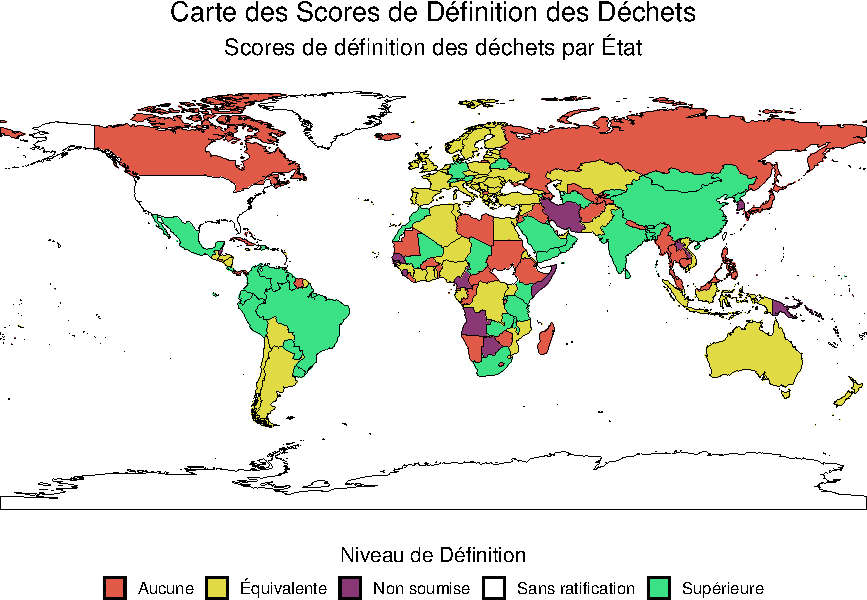
\includegraphics{Essai_JeanneDesrosiers_files/figure-latex/pressure1-1.pdf}

Outre les tendances continentales, face à la carte choroplèthe, il apparaît aisé d'observer des tendances régionales concernant l'émergence de définitions de la notion des déchets plus développées. En effet, le Nord de l'Amérique du Sud semble mener un effet d'entraînement sur le reste du continent. Malgré un certain conservatisme européen sur la définition, on observe un îlot en Europe centrale, possiblement une influence germanique pour des définitions plus ambitieuses. La péninsule arabique est principalement au vert. La région des Grands Lacs en Afrique semble être le principal centre de développement de la définition sur le continent. Finalement, un corridor Inde-Chine semble se dessiner, joignant l'Asie méridionale et l'Asie d'Extrême-Orient dans une opération de développement normatif.

\subsection{Référence à des concepts additionnels au sein du texte des définitions de niveau supérieur}\label{ruxe9fuxe9rence-uxe0-des-concepts-additionnels-au-sein-du-texte-des-duxe9finitions-de-niveau-supuxe9rieur}

La majorité du travail de redéfinition normative de la notion de déchets (57.14\%) est réalisé par des États d'Asie (33.33\%) ou d'Afrique (23.81\%). Si on ajoute les pays d'Amérique du Sud, qui arrive en troisième (19.05\%), on constate 76.19\% du travail normatif provient de ces trois régions du monde.

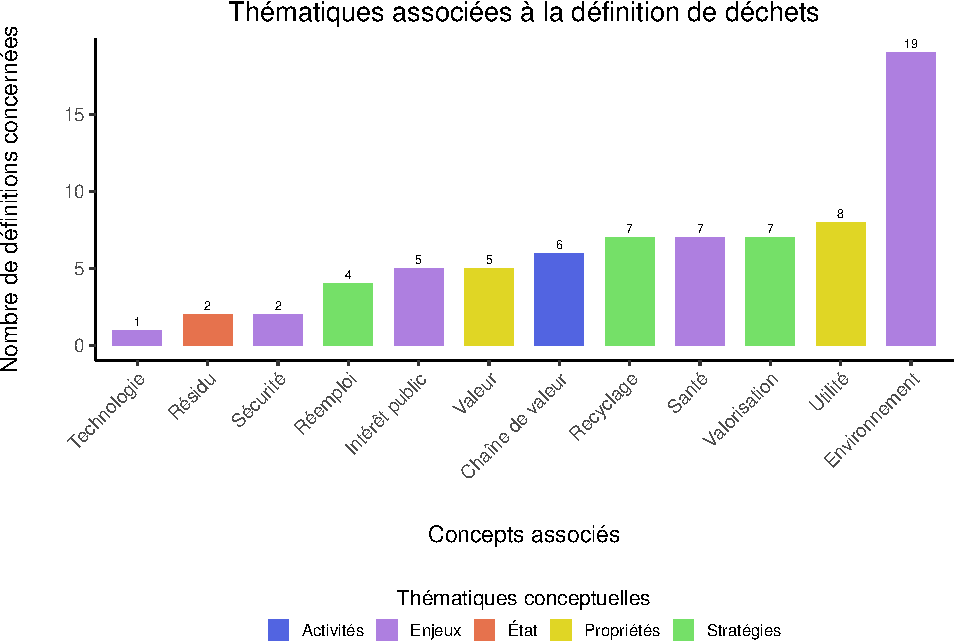
\includegraphics{Essai_JeanneDesrosiers_files/figure-latex/pressure2-1.pdf}

Ce travail de redéfinition normative se fait principalement par la fusion et le greffage normatifs et on remarque un arrimage sans pareil de la notion de déchet avec l'enjeu de l'environnement. En effet, 45.24\% des définitions dont le texte est plus demandant que celui de la Convention relient déchets et environnement, que ce soit par la mention de la pollution, des impacts environnementaux, des dangers pour les écosystèmes, etc. Ces conséquences environnementales relatives aux déchets se révèleraient ainsi être des préoccupations prioritaires chez ces États.

\subsection{Législations nationales mises en place pour assurer la conformité de la Convention}\label{luxe9gislations-nationales-mises-en-place-pour-assurer-la-conformituxe9-de-la-convention}

La production législative en matière de gestion des déchets liée à la Convention serait principalement concentrée en Europe (44.62\%), le reste étant distribué de manière variable dans le reste du monde (55.38\%). Cette intensité du travail législatif européen se traduit également dans la moyenne continentale de mesures par État, avec une moyenne dépassant de 94.72\% la moyenne mondiale fixée à 3.875 dispositions légales par État. Cette intensité de la production légale semble inverse à la production normative, où la moyenne européenne serait sous la moyenne mondiale de 48.32\%. Pour que ce qui est de l'Océanie, l'Amérique du Sud et l'Amérique du Nord, le tout semble constant avec les autres tendances observées plus haut. Cependant, pour l'Afrique et l'Asie, alors que les États de ces régions sont ceux qui ont réalisé la majorité du travail normatif sur la notion de déchets, l'Asie étant même à 32.64\% au-dessus de la moyenne mondiale de production normative, les deux régions continentales se trouvent au-dessous de la moyenne pour leur production législative, l'Asie à 13.98\% et l'Afrique à -55.69\%, les deux représentant au total 33.74\% des dispositions légales mises en place à l'échelle mondiale.

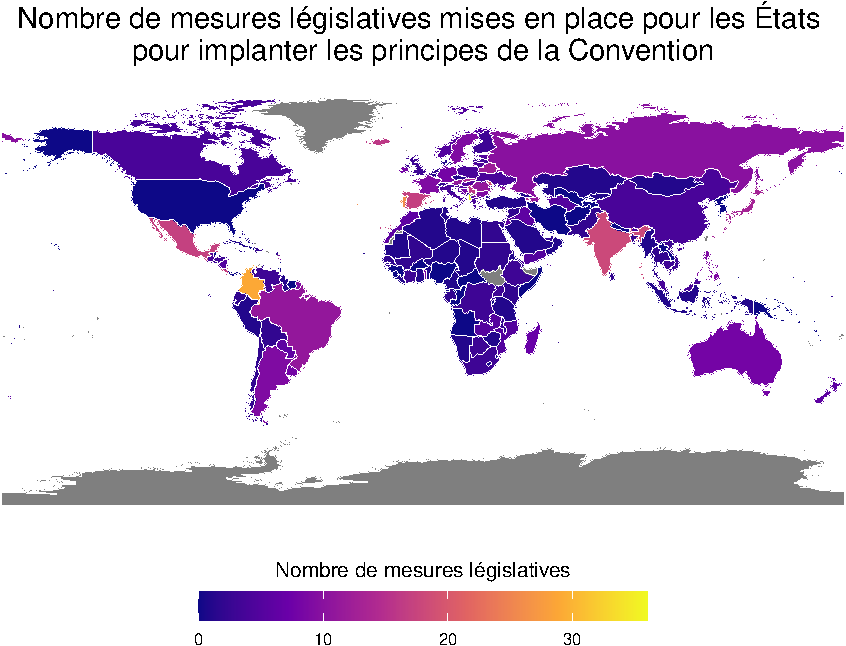
\includegraphics{Essai_JeanneDesrosiers_files/figure-latex/pressure3-1.pdf}

En observant la carte, on remarque rapidement que certains États se démarquent en étant largement au-dessus de la moyenne mondiale de production législative en lien avec la Convention de 3.875 dispositions. En effet, dépassant le cap du 10 dispositions légales, on retrouve, en ordre croissant, la Russie (10), la Roumanie (11), le Brésil (11), l'Azerbaïdjan (11), l'Autriche (11), la Dominique (12), le Biélorussie (12), le Japon (13), la Slovaquie (14), l'Arménie (15), la Serbie (16), l'Islande (16), l'Espagne (17), le Mexique (17), le Costa Rica (17), l'Inde (18), la Moldavie (19), le Portugal (26), la Colombie (29) et l'Albanie (36). De ces 20 États surperformants au comparatif en matière de production législative, on remarque que 40\% d'entre-eux ont une définition plus ambitieuse que celle de la Convention en matière de déchets. 35\% d'entre-eux ont une définition équivalente à celle de la Convention, 20\% n'ont pas définition de la notion de déchets et 5\% n'ont pas déclaré de définition.

\section{Discussion}\label{discussion}

Comme l'ont démontré les disparités en termes d'efforts normatifs et législatifs, il semblerait que la diffusion d'une norme sur la définition de la notion déchets ne soit pas stable à travers le monde (Busch \& Jörgens, 2005a, p. 86). La Figure 1 permet d'observer des tendances d'affinités régionales dans l'intensité des définitions adoptées et suggère que celles-ci se construiraient potentiellement sur le partage d'expériences communes dû à la proximité géographique (Amérique du Sud) ou à une situation économique similaire (corridor Inde-Chine), la participation à de mêmes familles légales ou culturelles (îlot germanique en Europe) ou la proximité avec un lieu influent sur la question (bassin des Grands Lacs et proximité avec l'UNEP) (Berkowitz et al., 2003, p. 166; Dobbin et al., 2007, pp. 449--461).

La pluralité (41.36\%) des États ont adopté une définition équivalente à celle de la Convention, ce qui permettrait d'assumer l'institutionnalisation de norme, selon l'idée de point de bascule au tiers des États (Finnemore \& Sikkink, 1998, p. 901). Cependant, il serait hâtif de considérer que la norme est internalisée, puisque, outre les États qui décident d'aller plus loin que la définition de la Convention, il reste que 36.65\% des États décident de ne pas participer au mécanisme déclaratoire concernant la définition de la notion de déchets ou déclarent ne pas définir cette notion nationalement.

De plus, le travail de redéfinition de la notion de déchets entrepris par les États qui choisissent de dépasser la proposition normative de la Convention démontre possiblement une entrée dans une nouvelle phase d'émergence normative pour la question des déchets. Par des processus de fusion et de greffage, les États concernés lient la notion de déchets avec d'autres concepts à travers leurs apprentissages et ceux de leurs voisins et les besoins qu'ils constatent sur leur territoire (Dobbin et al., 2007, pp. 449--461; Gönenç, 2021, p. 446; Watson, 1978, p. 332). Cela expliquerait pourquoi les pays du BRICS, par exemple, sont aussi mobilisés dans la définition de la notion de déchets, à l'exception de la Russie, par le partage d'une expérience commune. Cela expliquerait également l'implication des pays asiatiques et africains; étant les principales destinations des exports de déchets des pays développés, ils sont aux premières loges pour constater les impacts des déchets sur leur environnement, leurs populations et leur territoire. On pourrait faire l'hypothèse que sur cette question, l'Asie et l'Afrique font appel à un mécanisme inverse à celui de la compétition souvent observé lors de la diffusion de nouvelles normes pour abaisser les standards environnementaux pour faciliter la venue des capitaux extérieurs, par exemple. En effet, face à un sort commun qui nuit à leur développement, ces pays feraient peut-être de manière organisée ou non un front contre l'export de déchets sur leur territoire (Bernard, Claire, Vergne, \& Warin, 2014, p. 15; Marsh \& Sharman, 2009, pp. 271--272).

Il semblerait, et c'est possiblement la conclusion la plus intéressante de cet essai, que les efforts de redéfinition de la norme pour les déchets soient des démarches particulièrement clivantes sur la scène internationale, particulièrement dans les relations entre le Nord global et le Sud global (Hadden \& Seybert, 2016, p. 261; Stalley, 2018). En effet, la définition de base, celle de la Convention, est particulièrement peu exigeante, c'est-à-dire que la définition possède à la fois une composante objective et une composante subjective qui laisse ainsi beaucoup place à l'interprétation, mais surtout à une marge de manœuvre majeure pour les États ratificateurs. En soit, cette définition très «volontaire» des déchets n'est pas aberrante du fait de la tendance connue des traités environnementaux sur la pollution transfrontalière à manquer de profondeur. Elle s'inscrit également dans son époque, les années 90 représentant une montée du paradigme de l'approche volontaire dans la construction des accords internationaux (Amasuomo \& Baird, 2016, p. 89; Busch et al., 2005, pp. 146--148; Downs et al., 1996, p. 391; Wiprächtiger, Haupt, Rapp, \& Hellweg, 2021).

L'enjeu vient plutôt du constat qu'il semblerait y avoir une relation inverse entre le travail normatif, soit le développement de définitions plus ambitieuses sur les déchets, qui est principalement associé au Sud global, et le travail législatif, soit la mise en place de dispositions légales pour internaliser les principes existants de la Convention de Bâle, principalement associé quant à lui au Nord global. Cette différence notable semble confirmer la tendance des pays occidentaux à vouloir gérer un enjeu environnemental en maintenant leurs conditions existantes en contraste avec la tendance des pays non occidentaux à vouloir recadrer un enjeu pour générer des changements structurels. Dans le cadre de la question des déchets, on pourrait l'interpréter comme une opposition entre l'idée de la gestion des déchets et l'idée de la réduction des déchets. Cette dissociation des objectifs reliés au travail normatif et au travail législatif sur la question des déchets remet en question la conception du cycle de vie d'une norme. Alors que le travail normatif effectué pour bonifier la définition des déchets vise à changer le système et la portée de la Convention, la majorité des États poussant dans un même sens vers une meilleure prise en compte des impacts environnementaux de la production de déchets, le travail législatif par l'adoption de dispositions légales de plus en plus nombreuses vise plutôt à fixer ou stabiliser l'écosystème international autour d'une définition très ouverte de notion de déchets, possiblement pour conserver une absence de contraintes sur les activités économiques des États. Cette attitude serait en correspondance avec les observations de certains auteurs sur le fait que les déchets sont un enjeu fortement rattaché au syndrome du «pas dans ma cour», particulièrement chez les pays occidentaux comme le démontre leurs flux d'exportations de leurs déchets. Elle confirmerait également les observations de certains auteurs concernant l'imbrication de la question des déchets dans des dynamiques et des luttes post-coloniales, avec un Sud global qui manquerait de ressources pour implanter un cadre défendu par le Nord, le tout pouvant être associé à l'émergence même de la Convention dans un contexte conflictuel entre ces deux pôles. Ainsi, alors qu'à première vue, le travail législatif important réalisé pour implanter la Convention nationalement, concentré massivement en Europe et ce, malgré une très faible participation de l'Union européenne à la Convention, peut être interprété comme des efforts pour l'internalisation de la norme sur les déchets, celui-ci peut aussi être interprété comme une démarche active de blocage, une forme de résistance contre les efforts pour faire évoluer la définition de la notion de déchets. Ainsi, alors que les acteurs normatifs seraient des «pure norm entrepreneurs», selon la typologie de Bloomfield, ceux-ci ne compétitionnant pas entre eux, les acteurs législatifs pourraient, contrairement à un réflexe de les placer avec les précédents, se situer plutôt de l'autre côté du spectre. Sans être des «pure norm anti-preneurs» comme les États-Unis qui refusent de ratifier la Convention malgré l'avoir signé alors qu'ils sont les plus grands producteurs et exportateurs de déchets, les acteurs législatifs seraient plutôt des «creative resisters», qui participent à la norme, mais s'opposent à sa modification, évolution ou redéfinition {[}Ansari, Jamal, \& Ahmad (2019), 299 et 318-319; barsalou\_international\_2018, 895-897; Bernard et al. (2014), 12 et 15; Bloomfield (2016), 321-331; Donald (1992); Hadden \& Seybert (2016), 261; Peiry (2013); Stalley (2018){]}.

\section{Conclusions et limites}\label{conclusions-et-limites}

En réponse à l'hypothèse posée plus haut et en vue des résultats discutés, la norme reliée à la définition de la notion de déchets ne serait pas internalisée, sans toutefois être contestée, mais fait plutôt l'objet de résistance en lien avec sa redéfinition. Ces résultats remettent ainsi en question la possibilité de véritablement distinguer les phases du cycle de vie d'une norme. Le cas présent démontre qu'une norme peut être institutionnalisée et faire l'objet d'efforts de diffusion et d'internalisation, tout en voyant de nouvelles formes d'elle-même émerger et tenter d'être diffusées.

Face à la complexité de l'évolution de la norme relative à la définition des déchets, il semble approprié de faire suite aux conclusions de Bloomfield (Bloomfield, 2016) et de chercher à voir si plusieurs cycles peuvent co-exister sur des normes et si d'autres types de cycles que le cycle de vie existent, à l'instar du cycle de contestation qu'il propose. Face aux présentes observations, des recherches supplémentaires seraient nécessaires pour savoir si les tendances relevées sont propres à la Convention, au régime des déchets ou sont plutôt généralement associées aux questions environnementales. De plus, face à la plausible contradiction entre le travail législatif et le travail normatif effectués, il est nécessaire pour approfondir cette hypothèse de se pencher plus en profondeur sur le contenu des normes, politiques et réglementations développées par les États pour comprendre les objectifs et intérêts qui dirigent leurs prises de positions dans le cadre du régime international des déchets. Pour s'assurer d'avoir une compréhension globale du régime des déchets et des évolutions normatives en son sein sur la notion des déchets, l'exercice effectué ici devrait être répété pour les autres traités internationaux sur la question, mais également sur les accords régionaux pour approfondir la compréhension des dynamiques d'apprentissage dans la diffusion d'une norme. Finalement, malgré pour assurer une fiabilité, une réplicabilité et meilleure validité des résultats, une analyse comme celle réalisée plus haut nécessiterait un codage à plusieurs codeurs et une vérification subséquente des taux de fiabilité intercodeurs. L'essai ici se veut donc exploratoire, dans le but d'ouvrir la voie à des analyses plus poussées et rigoureuses de question de la définition des déchets.

Pour conclure, face à une visible multiplicité des compréhensions sur ce qui constitue un déchet à l'échelle internationale, il est possible de remettre en question l'efficacité de la définition de la Convention de Bâle à cadrer ce qui constitue ou non un déchet pour les États et ainsi à promouvoir une gestion des déchets raisonnée, mais surtout une réduction des déchets comme elle le souligne dans la Déclaration de Carthagène (Secretariat Of The Basel Convention, 2011). Ces questionnements sont notamment soutenus par l'avènement de nouvelles conventions régionales, comme la Convention de Bamako pour les États africains et la Convention de Waigani pour les États du Forum des îles pacifiques, qui soulèvent possiblement la question à savoir quelle est la meilleure échelle pour gérer une telle question environnementale (Bernard et al., 2014, p. 18; Donald, 1992; Habermas, 1998). Pour répondre aux impératifs de réduction des déchets et d'optimisation de l'utilisation des ressources pour lesquels plaident les Nations Unies, un resserrement de la norme sur la définition des déchets est nécessaire. Sans une évacuation de sa composante subjective, la définition ne peut être efficace pour endiguer l'enjeu de surproduction de déchets actuel et entamer une véritable transition vers une économie circulaire (Wiprächtiger et al., 2021, pp. 1--2). Une réflexion normative est ainsi nécessaire afin de repenser la notion de déchets, actuellement ancrée dans un modèle économique linéaire, pour atteindre les objectifs en matière de respect des limites planétaires (Sauvé, Bernard, \& Sloan, 2016, p. 53).

\backmatter

\chapter*{Bibliographie}\label{bibliographie}
\addcontentsline{toc}{chapter}{Bibliographie}

\markboth{References}{References}

\noindent

\setlength{\parindent}{-0.20in}
\setlength{\leftskip}{0.20in}
\setlength{\parskip}{8pt}

\phantomsection\label{refs}
\begin{CSLReferences}{1}{0}
\bibitem[\citeproctext]{ref-acharya_how_2004}
Acharya, A. (2004). How {Ideas} {Spread}: {Whose} {Norms} {Matter}? {Norm} {Localization} and {Institutional} {Change} in {Asian} {Regionalism}. \emph{International Organization}, \emph{58}(02). http://doi.org/\href{https://doi.org/10.1017/S0020818304582024}{10.1017/S0020818304582024}

\bibitem[\citeproctext]{ref-amasuomo_concept_2016}
Amasuomo, E., \& Baird, J. (2016). The {Concept} of {Waste} and {Waste} {Management}. \emph{Journal of Management and Sustainability}, \emph{6}(4), 88--96. http://doi.org/\href{https://doi.org/10.5539/jms.v6n4p88}{10.5539/jms.v6n4p88}

\bibitem[\citeproctext]{ref-ansari_basel_2019}
Ansari, A. H., Jamal, P., \& Ahmad, M. H. B. (2019). The {Basel} {Convention}: {Re}-{Visting} {Some} {Socio}-{Legal} {Issues} {Pertaining} to {Transboundary} {Movement} of {Hazardous} and {Other} {Wastes}. \emph{Journal of the Indian Law Institute}, \emph{61}(3), 295--322. Retrieved from \url{https://www.jstor.org/stable/27097370}

\bibitem[\citeproctext]{ref-bennett_what_1991}
Bennett, C. J. (1991). What {Is} {Policy} {Convergence} and {What} {Causes} {It}? \emph{British Journal of Political Science}, \emph{21}(2), 215--233. http://doi.org/\href{https://doi.org/10.1017/S0007123400006116}{10.1017/S0007123400006116}

\bibitem[\citeproctext]{ref-berkowitz_transplant_2003}
Berkowitz, D., Pistor, K., \& Richard, J.-F. (2003). The {Transplant} {Effect}. \emph{The American Journal of Comparative Law}, \emph{51}(1), 163--204. http://doi.org/\href{https://doi.org/10.2307/3649143}{10.2307/3649143}

\bibitem[\citeproctext]{ref-bernard_etat_2014}
Bernard, S., Claire, A., Vergne, G., \& Warin, T. (2014). Un état des lieux sur le commerce international des déchets. \emph{CIRANO For Discussion...} Retrieved from \url{https://ideas.repec.org//p/cir/cirtra/2014dt-01.html}

\bibitem[\citeproctext]{ref-blondeel_what_2019}
Blondeel, M., Colgan, J., \& Van De Graaf, T. (2019). What {Drives} {Norm} {Success}? {Evidence} from {Anti}--{Fossil} {Fuel} {Campaigns}. \emph{Global Environmental Politics}, \emph{19}(4), 63--84. http://doi.org/\href{https://doi.org/10.1162/glep_a_00528}{10.1162/glep\_a\_00528}

\bibitem[\citeproctext]{ref-bloomfield_norm_2016}
Bloomfield, A. (2016). Norm antipreneurs and theorising resistance to normative change. \emph{Review of International Studies}, \emph{42}(2), 310--333. http://doi.org/\href{https://doi.org/10.1017/S026021051500025X}{10.1017/S026021051500025X}

\bibitem[\citeproctext]{ref-brandi_when_2019}
Brandi, C., Blümer, D., \& Morin, J.-F. (2019). When {Do} {International} {Treaties} {Matter} for {Domestic} {Environmental} {Legislation}? \emph{Global Environmental Politics}, \emph{19}(4), 14--44. Retrieved from \url{https://muse.jhu.edu/pub/6/article/741671}

\bibitem[\citeproctext]{ref-busch_international_2005}
Busch, P.-O., \& Jörgens, H. (2005a). International patterns of environmental policy change and convergence. \emph{European Environment}, \emph{15}(2), 80--101. http://doi.org/\href{https://doi.org/10.1002/eet.374}{10.1002/eet.374}

\bibitem[\citeproctext]{ref-busch_international_2005-1}
Busch, P.-O., \& Jörgens, H. (2005b). The {International} {Sources} of {Policy} {Convergence}: {Explaining} the {Spread} of {Environmental} {Policy} {Innovations}. \emph{Journal of European Public Policy}, \emph{12}, 860--884. http://doi.org/\href{https://doi.org/10.1080/13501760500161514}{10.1080/13501760500161514}

\bibitem[\citeproctext]{ref-busch_global_2005}
Busch, P.-O., Jörgens, H., \& Tews, K. (2005). The {Global} {Diffusion} of {Regulatory} {Instruments}: {The} {Making} of a {New} {International} {Environmental} {Regime}. \emph{The ANNALS of the American Academy of Political and Social Science}, \emph{598}(1), 146--167. http://doi.org/\href{https://doi.org/10.1177/0002716204272355}{10.1177/0002716204272355}

\bibitem[\citeproctext]{ref-cheyne_fitting_1995}
Cheyne, I., \& Purdue, M. (1995). Fitting {Definition} to {Purpose}: {The} {Search} for a {Satisfactory} {Definition} of {Waste}. \emph{Journal of Environmental Law}, \emph{7}(2), 149--168. Retrieved from \url{https://heinonline.org/HOL/P?h=hein.journals/jenv7&i=155}

\bibitem[\citeproctext]{ref-circle_economy_leconomie_2024}
Circle Economy, \& RECYC-QUÉBEC. (2024). \emph{L'économie circulaire: Un outil pour respecter les limites planétaires} (Rapport complémentaire) (pp. 1--34). Québec. Retrieved from \url{https://www.recyc-quebec.gouv.qc.ca/sites/default/files/documents/rapport-limites-planetaires.pdf}

\bibitem[\citeproctext]{ref-daley_horizontal_2005}
Daley, D. M., \& Garand, J. C. (2005). Horizontal {Diffusion}, {Vertical} {Diffusion}, and {Internal} {Pressure} in {State} {Environmental} {Policymaking}, 1989-1998. \emph{American Politics Research}, \emph{33}(5), 615--644. http://doi.org/\href{https://doi.org/10.1177/1532673X04273416}{10.1177/1532673X04273416}

\bibitem[\citeproctext]{ref-dobbin_global_2007}
Dobbin, F., Simmons, B., \& Garrett, G. (2007). The {Global} {Diffusion} of {Public} {Policies}: {Social} {Construction}, {Coercion}, {Competition}, or {Learning}? \emph{Annual Review of Sociology}, \emph{33}(1), 449--472. http://doi.org/\href{https://doi.org/10.1146/annurev.soc.33.090106.142507}{10.1146/annurev.soc.33.090106.142507}

\bibitem[\citeproctext]{ref-dolowitz_learning_2000}
Dolowitz, D. P., \& Marsh, D. (2000). Learning from {Abroad}: {The} {Role} of {Policy} {Transfer} in {Contemporary} {Policy}-{Making}. \emph{Governance}, \emph{13}(1), 5--23. http://doi.org/\href{https://doi.org/10.1111/0952-1895.00121}{10.1111/0952-1895.00121}

\bibitem[\citeproctext]{ref-donald_bamako_1992}
Donald, J. W. (1992). The {Bamako} {Convention} as a {Solution} to the {Problem} of {Hazardous} {Waste} {Exports} to {Less} {Developed} {Countries}. \emph{Columbia Journal of Environmental Law}, \emph{17}, 419--458. Retrieved from \url{https://heinonline.org/HOL/Page?handle=hein.journals/cjel17&id=425&div=&collection=}

\bibitem[\citeproctext]{ref-downs_is_1996}
Downs, G. W., Rocke, D. M., \& Barsoom, P. N. (1996). Is the good news about compliance good news about cooperation? \emph{International Organization}, \emph{50}(3), 379--406. http://doi.org/\href{https://doi.org/10.1017/S0020818300033427}{10.1017/S0020818300033427}

\bibitem[\citeproctext]{ref-entman_framing_1993}
Entman, R. M. (1993). Framing: {Toward} {Clarification} of a {Fractured} {Paradigm}. \emph{Journal of Communication}, \emph{43}(4), 51--58. http://doi.org/\href{https://doi.org/10.1111/j.1460-2466.1993.tb01304.x}{10.1111/j.1460-2466.1993.tb01304.x}

\bibitem[\citeproctext]{ref-finnemore_international_1998}
Finnemore, M., \& Sikkink, K. (1998). International {Norm} {Dynamics} and {Political} {Change}. \emph{International Organization}, \emph{52}(4), 887--917. http://doi.org/\href{https://doi.org/10.1162/002081898550789}{10.1162/002081898550789}

\bibitem[\citeproctext]{ref-florini_evolution_1996}
Florini, A. (1996). The {Evolution} of {International} {Norms}. \emph{International Studies Quarterly}, \emph{40}(3), 363--389. http://doi.org/\href{https://doi.org/10.2307/2600716}{10.2307/2600716}

\bibitem[\citeproctext]{ref-gonenc_conceptualizing_2021}
Gönenç, D. (2021). Conceptualizing norm fusion through environmental rights. \emph{Environmental Politics}, \emph{30}(3), 442--461. http://doi.org/\href{https://doi.org/10.1080/09644016.2020.1743610}{10.1080/09644016.2020.1743610}

\bibitem[\citeproctext]{ref-haas_why_1979}
Haas, E. B. (1979). Why {Collaborate}? {Issue}-{Linkage} and {International} {Regimes}. \emph{World Politics}, \emph{32}(3), 357--405. Retrieved from \url{https://heinonline.org/HOL/P?h=hein.journals/wpot32&i=375}

\bibitem[\citeproctext]{ref-habermas_integration_1998}
Habermas, J. (1998). \emph{L'intégration républicaine : Essais de théorie politique}. Paris: Fayard.

\bibitem[\citeproctext]{ref-hadden_whats_2016}
Hadden, J., \& Seybert, L. A. (2016). What's in a {Norm}? {Mapping} the {Norm} {Definition} {Process} in the {Debate} on {Sustainable} {Development}. \emph{Global Governance: A Review of Multilateralism and International Organizations}, \emph{22}(2), 249--268. http://doi.org/\href{https://doi.org/10.1163/19426720-02202005}{10.1163/19426720-02202005}

\bibitem[\citeproctext]{ref-noauthor_international_2024}
International {Environmental} {Agreements} {Database} {Project}. (2024). Université Laval. Retrieved from \url{https://www.iea.ulaval.ca}

\bibitem[\citeproctext]{ref-loges_not_2020}
Loges, B., \& Jakobi, A. P. (2020). Not more than the sum of its parts: De-centered norm dynamics and the governance of plastics. \emph{Environmental Politics}, \emph{29}(6), 1004--1023. http://doi.org/\href{https://doi.org/10.1080/09644016.2019.1703385}{10.1080/09644016.2019.1703385}

\bibitem[\citeproctext]{ref-marsh_policy_2009}
Marsh, D., \& Sharman, J. C. (2009). Policy diffusion and policy transfer. \emph{Policy Studies}, \emph{30}(3), 269--288. http://doi.org/\href{https://doi.org/10.1080/01442870902863851}{10.1080/01442870902863851}

\bibitem[\citeproctext]{ref-marty_histoire_2023}
Marty, N., \& Druelle-Korn, C. (2023). Histoire des entreprises et économie circulaire : Pour une nécessaire clarification. \emph{Entreprises Et Histoire}, \emph{110}(1), 6--17. http://doi.org/\href{https://doi.org/10.3917/eh.110.0006}{10.3917/eh.110.0006}

\bibitem[\citeproctext]{ref-meadows_limits_1972}
Meadows, D. H., \& Club de Rome. (1972). \emph{The limits to growth: A report for the {Club} of {Rome}'s project on the predicament of mankind}. New York: Universe Books.

\bibitem[\citeproctext]{ref-moore_negotiating_2012}
Moore, F. C. (2012). Negotiating {Adaptation}: {Norm} {Selection} and {Hybridization} in {International} {Climate} {Negotiations}. \emph{Global Environmental Politics}, \emph{12}(4), 30--48. Retrieved from \url{https://muse.jhu.edu/pub/6/article/488275}

\bibitem[\citeproctext]{ref-organisation_des_nations_unies_objectif_nodate}
Organisation des Nations Unies. (n.d.). Objectif 12 : Établir des modes de consommation et de production durables. \emph{Nations Unies}. Retrieved from \url{https://www.un.org/sustainabledevelopment/fr/sustainable-consumption-production/}

\bibitem[\citeproctext]{ref-peiry_basel_2013}
Peiry, K. K. (2013). The {Basel} {Convention} on the {Control} of {Transboundary} {Movements} of {Hazardous} {Wastes} and their {Disposal}: {The} {Basel} {Convention} at a {Glance}. \emph{Proceedings of the ASIL Annual Meeting}, \emph{107}, 434--436. http://doi.org/\href{https://doi.org/10.5305/procannmeetasil.107.0434}{10.5305/procannmeetasil.107.0434}

\bibitem[\citeproctext]{ref-pongracz_evolving_2004}
Pongrácz, E., Phillips, P. S., \& Keiski, R. L. (2004). Evolving the {Theory} of {Waste} {Management}: {Defining} {Key} {Concepts}. In C. A. Brebbia, S. Kungolos, V. Popov, \& H. Itoh (Eds.), \emph{Waste {Management} and the {Environment} {II}} (WIT Press, Vol. 78, pp. 471--480). Retrieved from \url{https://www.witpress.com/elibrary/wit-transactions-on-ecology-and-the-environment/78/14399}

\bibitem[\citeproctext]{ref-price_reversing_1998}
Price, R. (1998). Reversing the {Gun} {Sights}: {Transnational} {Civil} {Society} {Targets} {Land} {Mines}. \emph{International Organization}, \emph{52}(3), 613--644. http://doi.org/\href{https://doi.org/10.1162/002081898550671}{10.1162/002081898550671}

\bibitem[\citeproctext]{ref-sauve_environmental_2016}
Sauvé, S., Bernard, S., \& Sloan, P. (2016). Environmental sciences, sustainable development and circular economy: {Alternative} concepts for trans-disciplinary research. \emph{Environmental Development}, \emph{17}, 48--56. http://doi.org/\href{https://doi.org/10.1016/j.envdev.2015.09.002}{10.1016/j.envdev.2015.09.002}

\bibitem[\citeproctext]{ref-secretariat_of_the_basel_convention_history_nodate}
Secretariat of the Basel Convention. (n.d.). History of the negotiations of the {Basel} {Convention}. \emph{Basel Convention on the Control of Transboundary Movements of Hazardous Wastes and their Disposal}. Retrieved from \url{https://www.basel.int/TheConvention/Overview/History/Overview/tabid/3405/Default.aspx}

\bibitem[\citeproctext]{ref-secretariat_of_the_basel_convention_cartagena_2011}
Secretariat Of The Basel Convention. (2011). \emph{Cartagena {Declaration} on the {Prevention}, {Minimization} and {Recovery} of {Hazardous} {Wastes} and {Other} {Wastes}} (pp. 1--3). Retrieved from \url{https://www.basel.int/Portals/4/Basel\%20Convention/docs/meetings/cop/cop10/CartagenaDeclaration.pdf}

\bibitem[\citeproctext]{ref-secretariat_of_the_basel_convention_basel_2023}
Secretariat Of The Basel Convention. (2023). \emph{Basel {Convention} on the {Control} of {Transboundary} {Movements} of {Hazardous} {Wastes} and their {Disposal}} (pp. 1--98). Retrieved from \url{https://www.basel.int/TheConvention/Overview/TextoftheConvention/tabid/1275/Default.aspx}

\bibitem[\citeproctext]{ref-setiawan_basel_2024}
Setiawan, F. A. (2024, September). \emph{The {Basel} {Convention} as an {Evolving} {Treaty} {Regime}: {Implications} of the {Ban} {Amendment} and {Plastic} {Waste} {Amendment}} (PhD thesis). Kobe University, Kobe. Retrieved from \url{https://hdl.handle.net/20.500.14094/0100477901}

\bibitem[\citeproctext]{ref-stalley_norms_2018}
Stalley, P. (2018). Norms from the periphery: Tracing the rise of the common but differentiated principle in international environmental politics. \emph{Cambridge Review of International Affairs}, \emph{31}(2), 141--161. http://doi.org/\href{https://doi.org/10.1080/09557571.2018.1481824}{10.1080/09557571.2018.1481824}

\bibitem[\citeproctext]{ref-terzi_emotional_2024}
Terzi, Ö. (2024). Emotional politics of norm hierarchy in {EU}'s external relations: The case of climate crisis and the {EU}'s arctic policy. \emph{Journal of European Integration}, \emph{46}(5), 729--749. http://doi.org/\href{https://doi.org/10.1080/07036337.2024.2359590}{10.1080/07036337.2024.2359590}

\bibitem[\citeproctext]{ref-watson_comparative_1978}
Watson, A. (1978). Comparative {Law} and {Legal} {Change}. \emph{The Cambridge Law Journal}, \emph{37}(2), 313--336. http://doi.org/\href{https://doi.org/10.1017/S0008197300093338}{10.1017/S0008197300093338}

\bibitem[\citeproctext]{ref-weiss_engaging_2000}
Weiss, E. B., \& Jacobson, H. K. (2000). \emph{Engaging {Countries}: {Strengthening} {Compliance} with {International} {Environmental} {Accords}}. MIT Press.

\bibitem[\citeproctext]{ref-wiener_theory_2014}
Wiener, A. (2014). \emph{A {Theory} of {Contestation}}. Berlin, Heidelberg: Springer. http://doi.org/\href{https://doi.org/10.1007/978-3-642-55235-9}{10.1007/978-3-642-55235-9}

\bibitem[\citeproctext]{ref-wiener_something_2000}
Wiener, J. B. (2000). Something {Borrowed} for {Something} {Blue}: {Legal} {Transplants} and the {Evolution} of {Global} {Environmental} {Law}. \emph{Ecology Law Quarterly}, \emph{27}(4), 1295--1372. Retrieved from \url{https://heinonline.org/HOL/P?h=hein.journals/eclawq27&i=1305}

\bibitem[\citeproctext]{ref-wiprachtiger_waste_2021}
Wiprächtiger, M., Haupt, M., Rapp, M., \& Hellweg, S. (2021). Waste not, want not -- ambiguities around waste and waste prevention. \emph{Resources, Conservation and Recycling}, \emph{173}, 105742. http://doi.org/\href{https://doi.org/10.1016/j.resconrec.2021.105742}{10.1016/j.resconrec.2021.105742}

\end{CSLReferences}


% Index?

\end{document}
